\chapter{LDPC Decoder Design} \label{ch:LDPCdec}

\emph{This chapter is an addendum written in 2026, after the thesis was discussed in July 2008. The thesis designed the transmitter side of the DVB-S2 FEC: the BCH encoder of Chapters~\ref{ch:BCHencImpl} and~\ref{ch:SWForVDL} and the interface to the LDPC encoder. Section~\ref{sec:LDPCstruct} described the LDPC decoder only qualitatively. This chapter completes the picture on the receiver side: it derives the decoding algorithm, simplifies it for hardware, exploits the structure of the DVB-S2 code to obtain a 360-parallel architecture, and sizes word lengths, memories and throughput. All numbers come from the \texttt{dvbs2} Python package in the \texttt{sim/} directory of the repository: the modules \texttt{codes/ldpc.py} and \texttt{codes/ldpc\_hw.py}, the study \texttt{tools/ldpc\_study.py} and the figures \texttt{tools/ldpc\_figures.py}. Every simulated point runs the complete DVB-S2 link (BBFRAME, BCH, LDPC, bit interleaver, mapper, PLFRAME, AWGN channel, exact demapper and BCH decoder) for up to 50 frame errors or the number of frames given in the text.}

\section{Soft Information}

Let \(\vet c = (c_0 \virgola \ldots \virgola c_{N-1})\) be an LDPC codeword with \(\vet H \vet c\ap{T} = \vet 0\), \(\vet H\) the \((N-K) \times N\) parity-check matrix of Section~\ref{sec:LDPCstruct} and Figure~\ref{fig:Tanner}. The decoder does not see the bits. After the bit interleaver and the mapper of Section~\ref{sec:ACMdesc}, each bit travels in the label of a constellation symbol, and the demapper turns each received symbol \(y\) into one \emph{log-likelihood ratio} (LLR) per label bit:
\begin{equation} \label{eq:ldpc-llr}
\lambda_v = \ln \frac{P(c_v = 0 \mid y)}{P(c_v = 1 \mid y)} = \ln \frac{\sum_{s \in \mathcal{X}_0^i} e^{-|y - s|^2 / N_0}}{\sum_{s \in \mathcal{X}_1^i} e^{-|y - s|^2 / N_0}}
\end{equation}
where \(\mathcal{X}_b^i\) is the set of constellation points whose \(i\)-th label bit is \(b\) and equiprobable bits are assumed. The sign of \(\lambda_v\) is the hard decision (\(\lambda_v > 0\) means \(c_v = 0\)) and its magnitude is the reliability. The \emph{max-log} demapper keeps only the largest term of each sum,
\begin{equation} \label{eq:ldpc-maxlog}
\lambda_v \approx \frac{1}{N_0}\left( \min_{s \in \mathcal{X}_1^i} |y-s|^2 - \min_{s \in \mathcal{X}_0^i} |y-s|^2 \right)
\end{equation}
which needs no exponentials. For binary antipodal signalling with noise variance \(\sigma^2\) per dimension, (\ref{eq:ldpc-llr}) reduces to \(\lambda_v = 2 y_v / \sigma^2\). Bit-interleaved coded modulation (Section~\ref{sec:BICMintro}) is exactly this separation: whatever the constellation, the LDPC decoder only sees one LLR per code bit.

\section{Belief Propagation} \label{sec:ldpc-bp}

Let \(\mathcal{N}(v)\) be the checks of bit \(v\) (the 1s in column \(v\) of \(\vet H\)) and \(\mathcal{N}(c)\) the bits of check \(c\) (the 1s in row \(c\)). Belief propagation, also called the sum-product algorithm \cite{b:FactorGraphs, b:LDPCGall, b:MacKay}, exchanges LLRs along the edges of the Tanner graph: \(Q_{v \to c}\) from bit to check and \(R_{c \to v}\) from check to bit. Each message is \emph{extrinsic}: the message sent along an edge never uses the message that arrived along the same edge.

\paragraph{Variable nodes.} If the incoming opinions are independent, their log-likelihoods add:
\begin{equation} \label{eq:ldpc-vn}
Q_{v \to c} = \lambda_v + \sum_{c' \in \mathcal{N}(v) \setminus c} R_{c' \to v} \virgola \qquad L_v = \lambda_v + \sum_{c \in \mathcal{N}(v)} R_{c \to v}
\end{equation}
where \(L_v\) is the a posteriori LLR used for the decision. Note that \(Q_{v \to c} = L_v - R_{c \to v}\). This identity is the key to the layered decoder of Section~\ref{sec:ldpc-layered}.

\paragraph{Check nodes.} A check is satisfied when the modulo-2 sum of its bits is zero, so it tells bit \(v\) to equal the sum of the others. Gallager's lemma \cite{b:LDPCGall} gives the probability that a sum of independent bits with \(P(x_i = 1) = p_i\) is even:
\begin{equation} \label{eq:ldpc-gallager}
P\Big(\bigoplus_i x_i = 0\Big) = \frac{1}{2} + \frac{1}{2} \prod_i (1 - 2 p_i)
\end{equation}
For two bits this is \((1-p_1)(1-p_2) + p_1 p_2\), and induction extends it to any number of bits. With \(p = 1/(1 + e^{Q})\) we have \(1 - 2p = \tanh(Q/2)\). The LLR of the event "the other bits sum to 0" is then \(\ln \frac{1 + \Pi}{1 - \Pi} = 2\,\mathrm{atanh}\,\Pi\), where \(\Pi\) is the product, and therefore
\begin{equation} \label{eq:ldpc-tanh}
\tanh \frac{R_{c \to v}}{2} = \prod_{v' \in \mathcal{N}(c) \setminus v} \tanh \frac{Q_{v' \to c}}{2}
\end{equation}
Splitting signs and magnitudes, and taking logarithms of the magnitudes,
\begin{equation} \label{eq:ldpc-phi}
R_{c \to v} = \Big( \prod_{v' \in \mathcal{N}(c) \setminus v} \mathrm{sign}\, Q_{v' \to c} \Big) \; \phi\Big( \sum_{v' \in \mathcal{N}(c) \setminus v} \phi\big(|Q_{v' \to c}|\big) \Big)
\end{equation}
where
\begin{equation} \label{eq:ldpc-phidef}
\phi(x) = -\ln \tanh \frac{x}{2} = \ln \frac{e^x + 1}{e^x - 1}
\end{equation}
is its own inverse: if \(y = \phi(x)\) then \(\tanh(y/2) = (1 - e^{-y})/(1 + e^{-y}) = (1 - \tanh(x/2))/(1 + \tanh(x/2)) = e^{-x}\), that is \(\phi(y) = x\). Figure~\ref{fig:ldpc-checknode} (left) shows \(\phi\). It is large near 0 and decays quickly, so the sum in (\ref{eq:ldpc-phi}) is dominated by the least reliable inputs. The pairwise form of (\ref{eq:ldpc-tanh}) is often written with the "box-plus" operator,
\begin{equation} \label{eq:ldpc-boxplus}
\begin{aligned}
a \boxplus b &= 2\,\mathrm{atanh}\big(\tanh\tfrac{a}{2} \tanh\tfrac{b}{2}\big) \\
&= \mathrm{sign}(a)\,\mathrm{sign}(b) \min(|a|,|b|) + \ln\big(1 + e^{-|a+b|}\big) - \ln\big(1 + e^{-|a-b|}\big)
\end{aligned}
\end{equation}
and a check of degree \(d_c\) computes \(R_{c \to v} = \boxplus_{v' \ne v} Q_{v' \to c}\).

\paragraph{Schedule and stopping.} In the \emph{flooding} schedule all checks are updated from the same set of variable messages, then all variables, and this alternation is one iteration. After each iteration the decoder takes \(\hat c_v = 1\) if \(L_v < 0\) and stops as soon as \(\vet H \hat{\vet c}\ap{T} = \vet 0\). This syndrome test is the reason LDPC decoders know when they have finished, and most frames finish long before the iteration limit (Section~\ref{sec:ldpc-layered}). Belief propagation is exact on a graph without cycles. The DVB-S2 graphs have cycles, so the messages are only approximately independent, but the approximation is good when the cycles are long compared with the number of iterations.

\paragraph{Cost.} Each iteration evaluates two messages per edge of the graph. The DVB-S2 codes have \(E = \) 194\,399 to 285\,119 edges for normal frames (Table~\ref{tb:ldpc-structure}), so a decoder that runs 30 iterations on a 64\,800-bit frame computes more than \(10^7\) messages per frame. A flooding decoder also stores two messages per edge. Making this affordable is the subject of the rest of the chapter: cheaper check nodes (Section~\ref{sec:ldpc-minsum}), a better schedule (Section~\ref{sec:ldpc-layered}), and a code structure that maps onto parallel hardware (Section~\ref{sec:ldpc-qc}).

\begin{figure} \centering
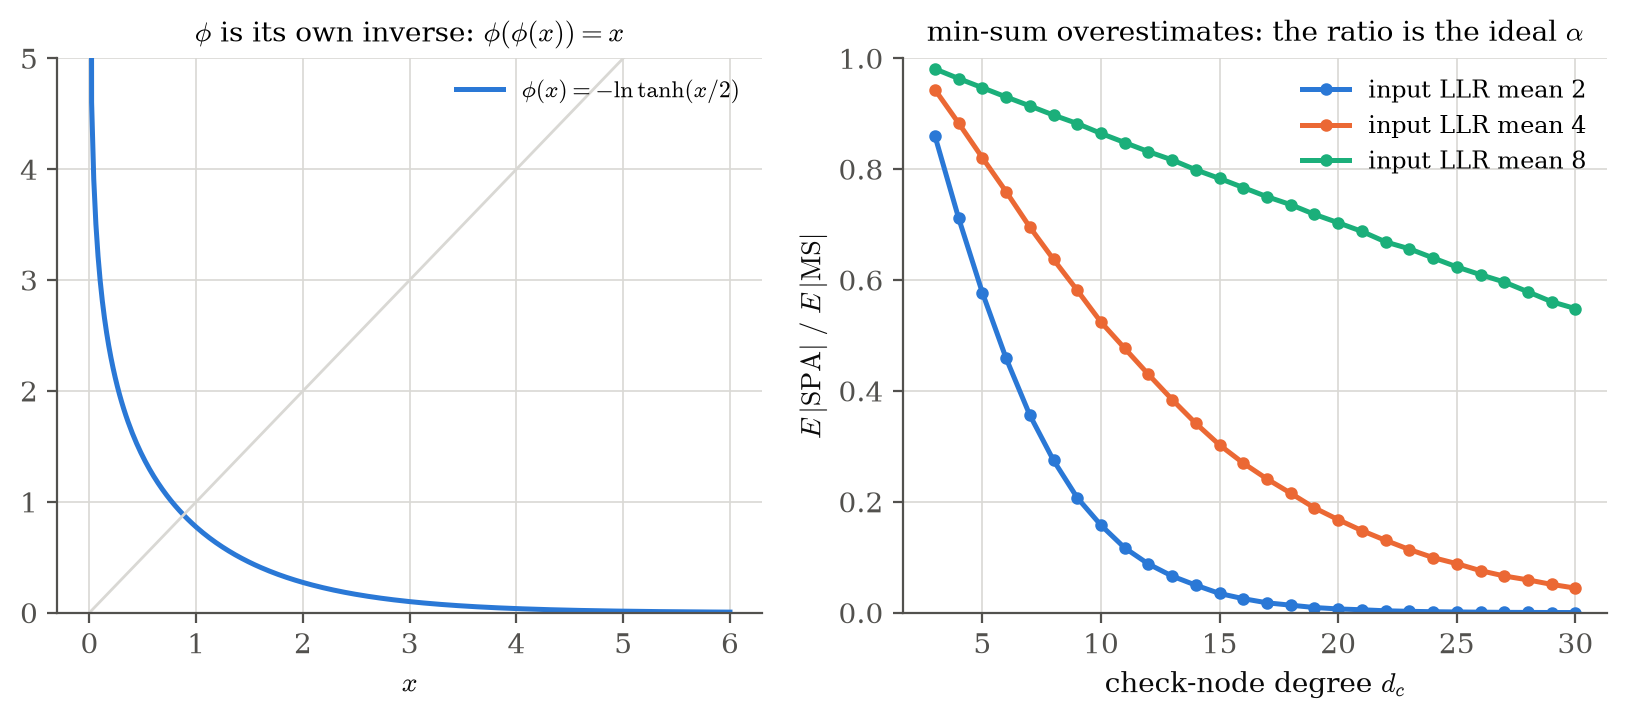
\includegraphics[width=\linewidth]{figures/ldpc-checknode.png}
\caption{Left: the function \(\phi(x) = -\ln\tanh(x/2)\) of the check-node update (\ref{eq:ldpc-phi}), which is its own inverse. Right: the ratio between the mean magnitude of the exact check-node output and the min-sum output, for \(d_c - 1\) Gaussian input LLRs with mean \(m\) and variance \(2m\). The ratio is the normalization \(\alpha\) that would make min-sum unbiased. It falls with the check degree and rises with the reliability of the inputs, so no single constant is right everywhere.} \label{fig:ldpc-checknode}
\end{figure}

\section{Reduced-Complexity Check Nodes} \label{sec:ldpc-minsum}

\paragraph{Min-sum.} Since \(\phi\) is positive and decreasing, the sum in (\ref{eq:ldpc-phi}) is at least its largest term \(\phi(\min_{v'} |Q_{v' \to c}|)\). Applying \(\phi\) once more reverses the inequality:
\begin{equation} \label{eq:ldpc-minsum}
|R_{c \to v}| = \phi\Big(\sum_{v'} \phi(|Q_{v' \to c}|)\Big) \le \min_{v' \in \mathcal{N}(c) \setminus v} |Q_{v' \to c}| = |R\ap{MS}_{c \to v}|
\end{equation}
The \emph{min-sum} algorithm uses the right-hand side directly: the sign product times the smallest input magnitude. It needs only comparisons, it is insensitive to a scaling of the LLRs (so the demapper need not know \(N_0\) exactly), and it always \emph{overestimates} the reliability of the check messages. Figure~\ref{fig:ldpc-checknode} (right) measures how much: the overestimation grows with the check degree, because more inputs push the true value down while the minimum stays put, and it shrinks as the inputs become reliable.

\paragraph{Corrections.} Two one-parameter corrections are used in practice \cite{b:ChenFossorier}:
\begin{equation} \label{eq:ldpc-corrections}
|R\ap{NMS}_{c \to v}| = \alpha \min_{v'} |Q_{v' \to c}| \virgola \qquad |R\ap{OMS}_{c \to v}| = \max\Big(\min_{v'} |Q_{v' \to c}| - \beta \virgola 0\Big)
\end{equation}
\emph{Normalized} min-sum (NMS) scales by \(0 < \alpha \le 1\). \emph{Offset} min-sum (OMS) subtracts \(\beta \ge 0\) and clips at zero. Both are cheap in hardware: \(\alpha = 1 - 2^{-k}\) is a shift and a subtraction, and \(\beta\) is a small integer in fixed point.

\begin{figure} \centering
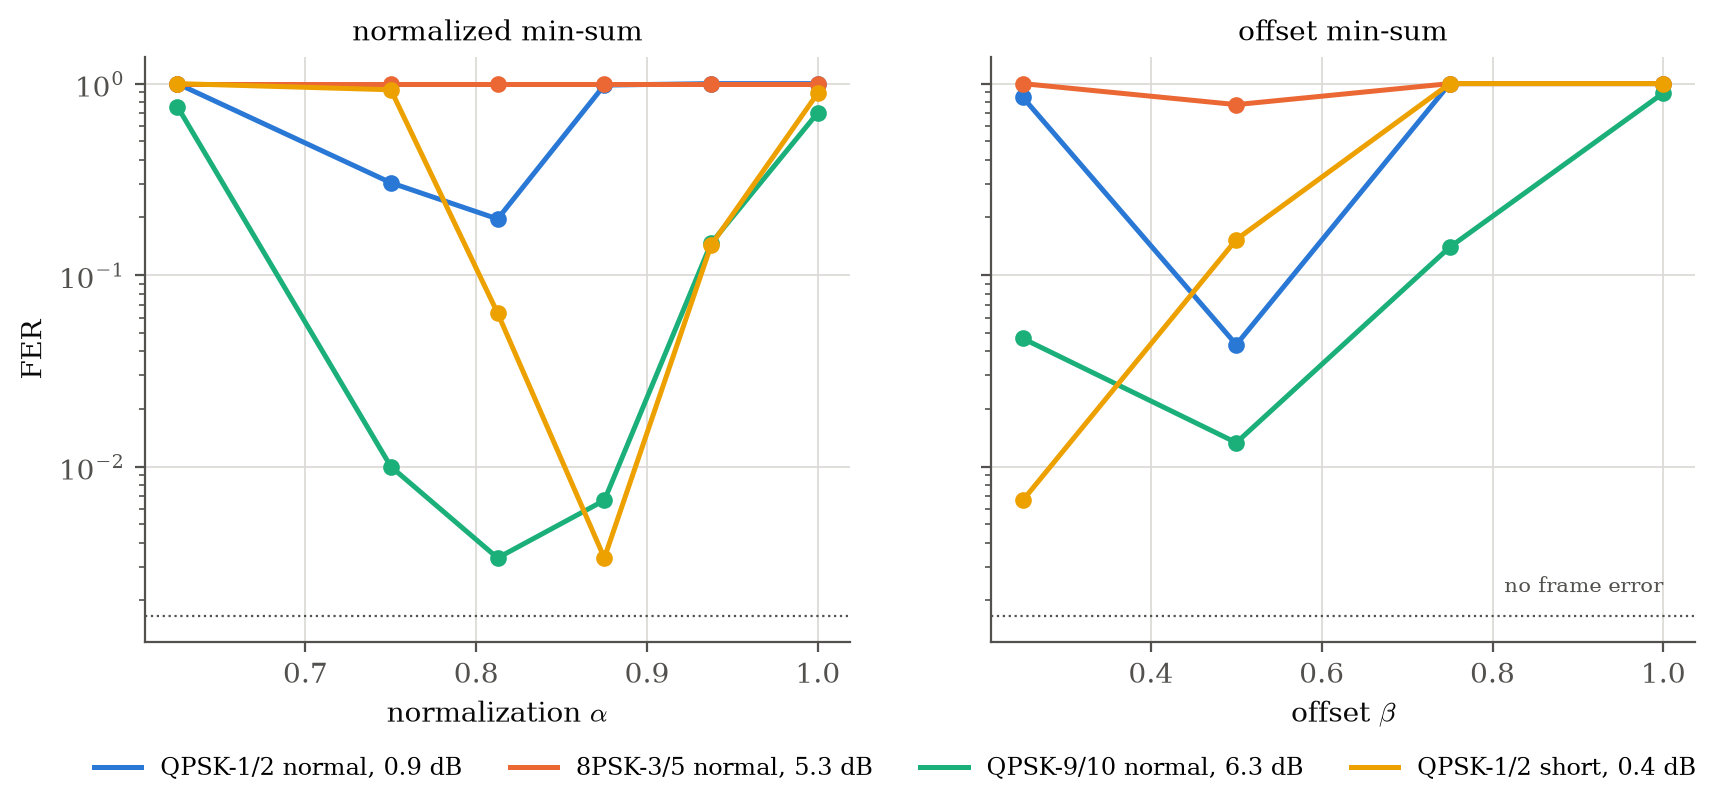
\includegraphics[width=\linewidth]{figures/ldpc-correction.png}
\caption{Frame error rate of normalized (left) and offset (right) min-sum versus the correction parameter, at the \(E_s/N_0\) where the sum-product decoder first reaches FER \(< 10^{-2}\) (layered schedule, 50 iterations, up to 300 frames per point; open markers: no frame error). \(\alpha = 1\) is plain min-sum.} \label{fig:ldpc-correction}
\end{figure}

Figure~\ref{fig:ldpc-correction} sweeps both parameters on four DVB-S2 MODCODs at the point where sum-product decoding has just reached FER \(= 10^{-2}\). Three facts stand out.
\begin{enumerate}
\item \emph{A correction is necessary.} Plain min-sum (\(\alpha = 1\)) fails at all four points.
\item \emph{Normalization is fragile on these codes.} The useful range of \(\alpha\) is narrow and depends on the code: \(0.8125\) is best for QPSK 1/2 and 9/10 normal frames, \(0.875\) for the short QPSK 1/2 frame, and one step away from the best value most frames are lost: on QPSK 1/2 normal frames the FER is 0.20 at \(\alpha = 0.8125\) but 0.30 at 0.75 and 0.98 at 0.875, and on the short frame 0.003 at 0.875 but 0.93 at 0.75. On 8PSK 3/5 no normalization reaches the sum-product threshold at all. In the frames that fail with a small \(\alpha\), 76\% of the wrong bits are degree-2 parity bits of the staircase and almost all the others are degree-3 information bits (measured on 40 frames of the short rate 1/2 code over a binary-input AWGN channel at \(E_b/N_0 = 1.6\) dB with \(\alpha = 0.7\)). An interpretation is that the staircase is a long chain of degree-2 nodes along which reliability must travel from check to check: a factor \(\alpha\) applied at every check attenuates it geometrically, as \(\alpha^k\) after \(k\) steps, while an offset only removes a constant from the small, unreliable messages and leaves the large ones almost untouched.
\item \emph{Offset min-sum has a stable optimum.} \(\beta = 0.5\) is the best offset for the three normal-frame codes; the short frame prefers 0.25. Too large an offset (\(\beta \ge 0.75\)) fails as badly as too small an \(\alpha\).
\end{enumerate}
A single operating point is a harsh test, however, because the waterfalls are steep. Figure~\ref{fig:ldpc-algorithms} compares the complete waterfalls with \(\alpha = 0.8125\) and \(\beta = 0.5\) on every code, and Table~\ref{tb:ldpc-thresholds} lists the \(E_s/N_0\) at which each decoder reaches FER \(< 10^{-2}\).

\begin{figure} \centering
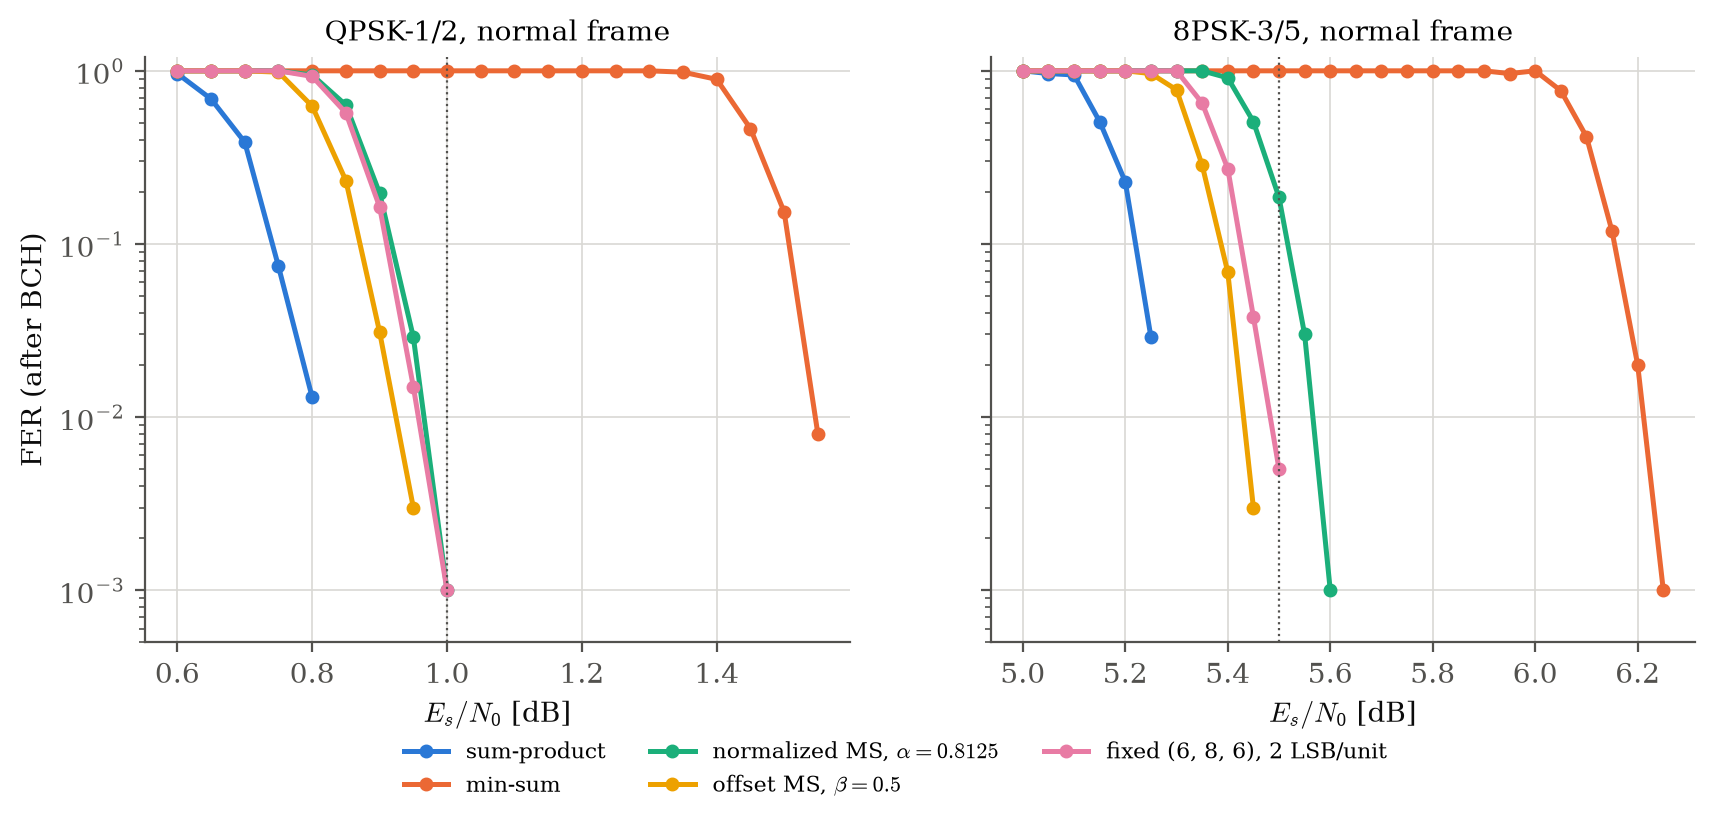
\includegraphics[width=\linewidth]{figures/ldpc-algorithms.png}
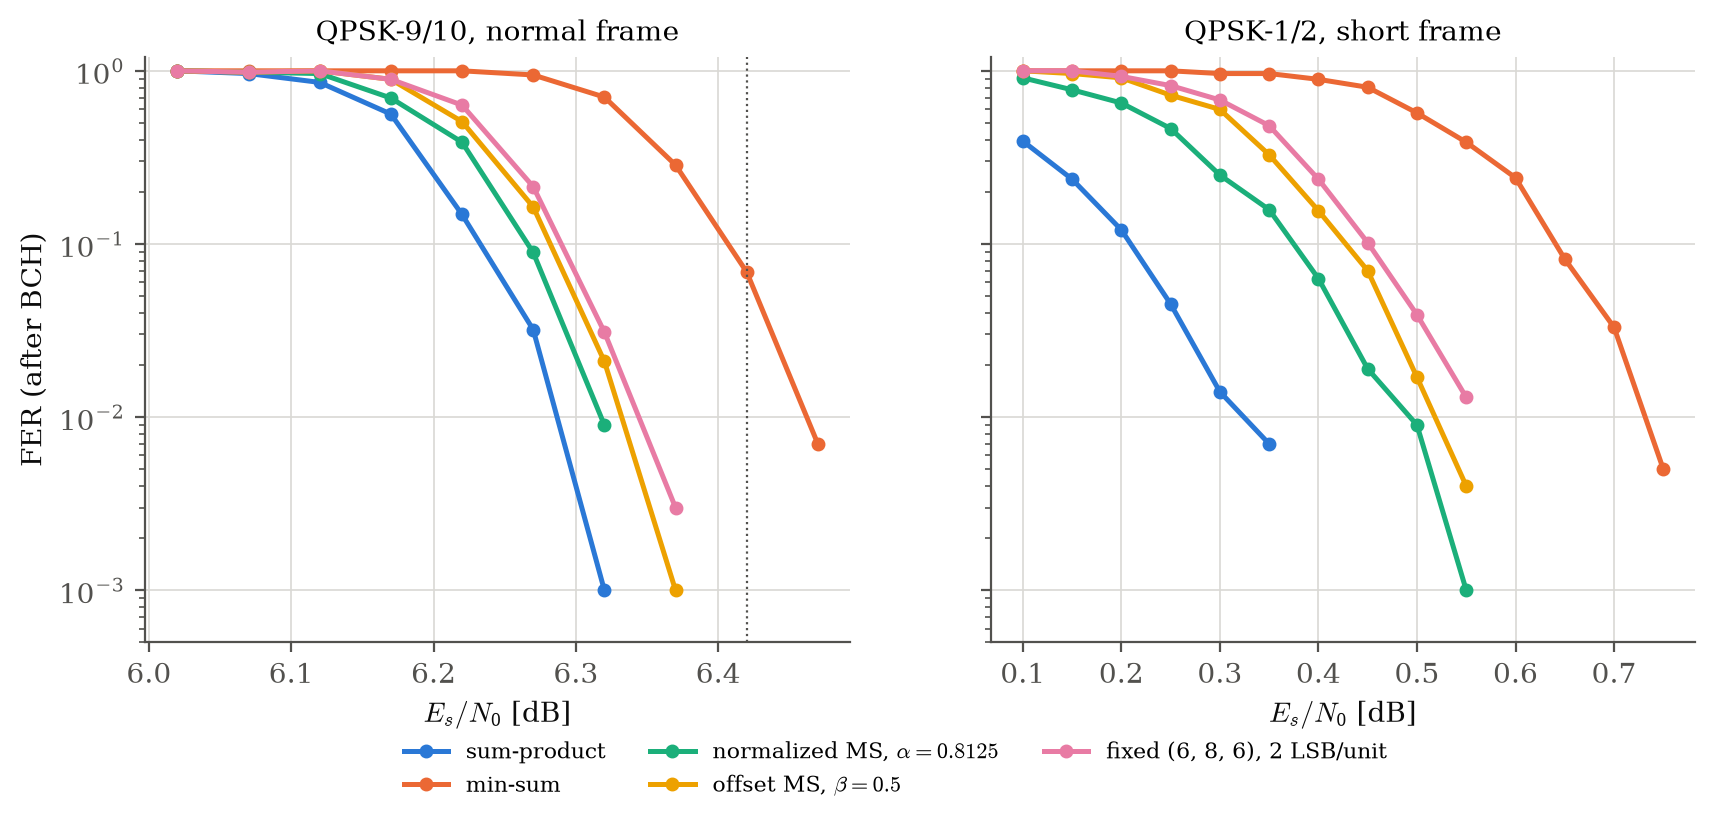
\includegraphics[width=\linewidth]{figures/ldpc-algorithms-2.png}
\caption{Frame error rate after BCH decoding of the full DVB-S2 link for sum-product, plain min-sum, normalized (\(\alpha = 0.8125\)) and offset (\(\beta = 0.5\)) min-sum and the fixed-point decoder of Section~\ref{sec:ldpc-fixed}. Layered schedule, 50 iterations. The dotted lines are the quasi-error-free \(E_s/N_0\) of EN 302 307 for normal frames.} \label{fig:ldpc-algorithms}
\end{figure}

\begin{table} \centering
\small \setlength{\tabcolsep}{4pt}
\begin{tabular}{|l|c|c|c|c|c|}
\hline
MODCOD & SPA & MS & NMS 0.8125 & OMS 0.5 & fixed \\
\hline
QPSK 1/2 normal & 0.85 & 1.55 (+0.70) & 1.00 (+0.15) & 0.95 (+0.10) & 1.00 (+0.15) \\
8PSK 3/5 normal & 5.30 & 6.25 (+0.95) & 5.60 (+0.30) & 5.45 (+0.15) & 5.50 (+0.20) \\
QPSK 9/10 normal & 6.32 & 6.47 (+0.15) & 6.32 (+0.00) & 6.37 (+0.05) & 6.37 (+0.05) \\
QPSK 1/2 short & 0.35 & 0.75 (+0.40) & 0.50 (+0.15) & 0.55 (+0.20) & 0.60 (+0.25) \\
\hline
\end{tabular}
\caption{\(E_s/N_0\) [dB] at which the frame error rate after BCH first falls below \(10^{-2}\) for sum-product (SPA), min-sum (MS), normalized min-sum with \(\alpha = 0.8125\), offset min-sum with \(\beta = 0.5\) and the \((6, 8, 6)\) fixed-point decoder at \(s = 2\) with an offset of 1 LSB (at \(s = 4\) its loss disappears, Section~\ref{sec:ldpc-fixed}) (layered schedule, 50 iterations, 0.05 dB steps, up to 1000 frames per point). In brackets: the loss with respect to sum-product.} \label{tb:ldpc-thresholds}
\end{table}

Table~\ref{tb:ldpc-thresholds} quantifies the losses. Plain min-sum costs 0.15 dB at rate 9/10, where the check degree is 30 and the messages are very reliable when the decoder converges, and 0.40--0.95 dB at the lower rates. Both corrections recover most of this. Offset min-sum stays within 0.10--0.20 dB of sum-product on all four codes. Normalized min-sum with \(\alpha = 0.8125\) is better on the rate 9/10 code (no loss) and on the short frame, and worse on 8PSK 3/5 (0.30 dB). Neither correction is uniformly better. Offset min-sum is chosen here because its best parameter is the same for the three normal-frame codes, because the waterfalls are steep enough that a fixed \(\beta\) is safe over the whole operating range, and because, as Section~\ref{sec:ldpc-fixed} shows, the offset is also what a fixed-point implementation of the normalization ends up doing. The waterfalls of 64\,800-bit frames are very steep: every decoder goes from FER \(\approx 1\) to below \(10^{-3}\) within about 0.3 dB, so a loss of 0.1 dB is a large fraction of the waterfall.

\paragraph{Compressed check-node state.} Min-sum has a second advantage, which matters more than the comparators. All the messages that check \(c\) sends are one of two magnitudes: the smallest input magnitude \(m_1\), sent to every bit except the one that supplied it, and the second smallest \(m_2\), sent to that bit. The signs are the total sign product times each input sign. The whole output of a check is therefore described by
\begin{equation} \label{eq:ldpc-compressed}
\big(m_1 \virgola m_2 \virgola \mathrm{idx}(m_1) \virgola \mathrm{sign}_1 \virgola \ldots \virgola \mathrm{sign}_{d_c}\big) \qquad \text{in } 2(w_R - 1) + \lceil \log_2 d_c \rceil + d_c \text{ bits}
\end{equation}
instead of \(d_c\) messages of \(w_R\) bits. For the rate 1/2 normal code (\(d_c = 7\), \(w_R = 6\)) this is 20 bits instead of 42 per check. Over all codes the check-message memory shrinks by a factor of 1.5 to 4 (Table~\ref{tb:ldpc-memory}). Sum-product has no such compression, because every output magnitude is different.

\section{Layered Decoding} \label{sec:ldpc-layered}

Flooding is the textbook schedule but not the best one. The identity \(Q_{v \to c} = L_v - R_{c \to v}\) of (\ref{eq:ldpc-vn}) suggests another one \cite{b:MansourShanbhag, b:Hocevar}. The decoder keeps only the posteriors \(L_v\) (initialized to \(\lambda_v\)) and the check messages \(R_{c \to v}\) (initialized to 0), and processes the checks one group (\emph{layer}) at a time:
\begin{align}
Q_{v \to c} &= L_v - R_{c \to v}\ap{old} && v \in \mathcal{N}(c) \label{eq:ldpc-layer1}\\
R_{c \to v}\ap{new} &= \mathrm{CN}\big(\{Q_{v' \to c}\}_{v' \ne v}\big) && \label{eq:ldpc-layer2}\\
L_v &= Q_{v \to c} + R_{c \to v}\ap{new} = L_v + \big(R_{c \to v}\ap{new} - R_{c \to v}\ap{old}\big) \label{eq:ldpc-layer3}
\end{align}
where CN is the check-node rule, (\ref{eq:ldpc-phi}) for sum-product or (\ref{eq:ldpc-corrections}) for min-sum. After each update \(L_v = \lambda_v + \sum_c R_{c \to v}\) still holds, with the most recent message of every check, so the bookkeeping is exact. The difference from flooding is that a check processed later in the same iteration already sees the messages that earlier checks produced in this iteration. Flooding and layered decoding relate to each other like the Jacobi and Gauss-Seidel iterations of linear algebra. Layered decoding also saves memory, because it needs no variable-to-check message memory: \(Q\) exists only inside the check-node processor, between (\ref{eq:ldpc-layer1}) and (\ref{eq:ldpc-layer3}).

Checks that share no bit can be updated at the same time without changing the result. In the DVB-S2 codes the 360 checks of a layer are of this kind (Section~\ref{sec:ldpc-qc}), apart from a few exceptions that are resolved by the second form of (\ref{eq:ldpc-layer3}): when one bit meets two checks of the same layer, both read the same \(L_v\), and both message changes are added to it.

\begin{figure} \centering
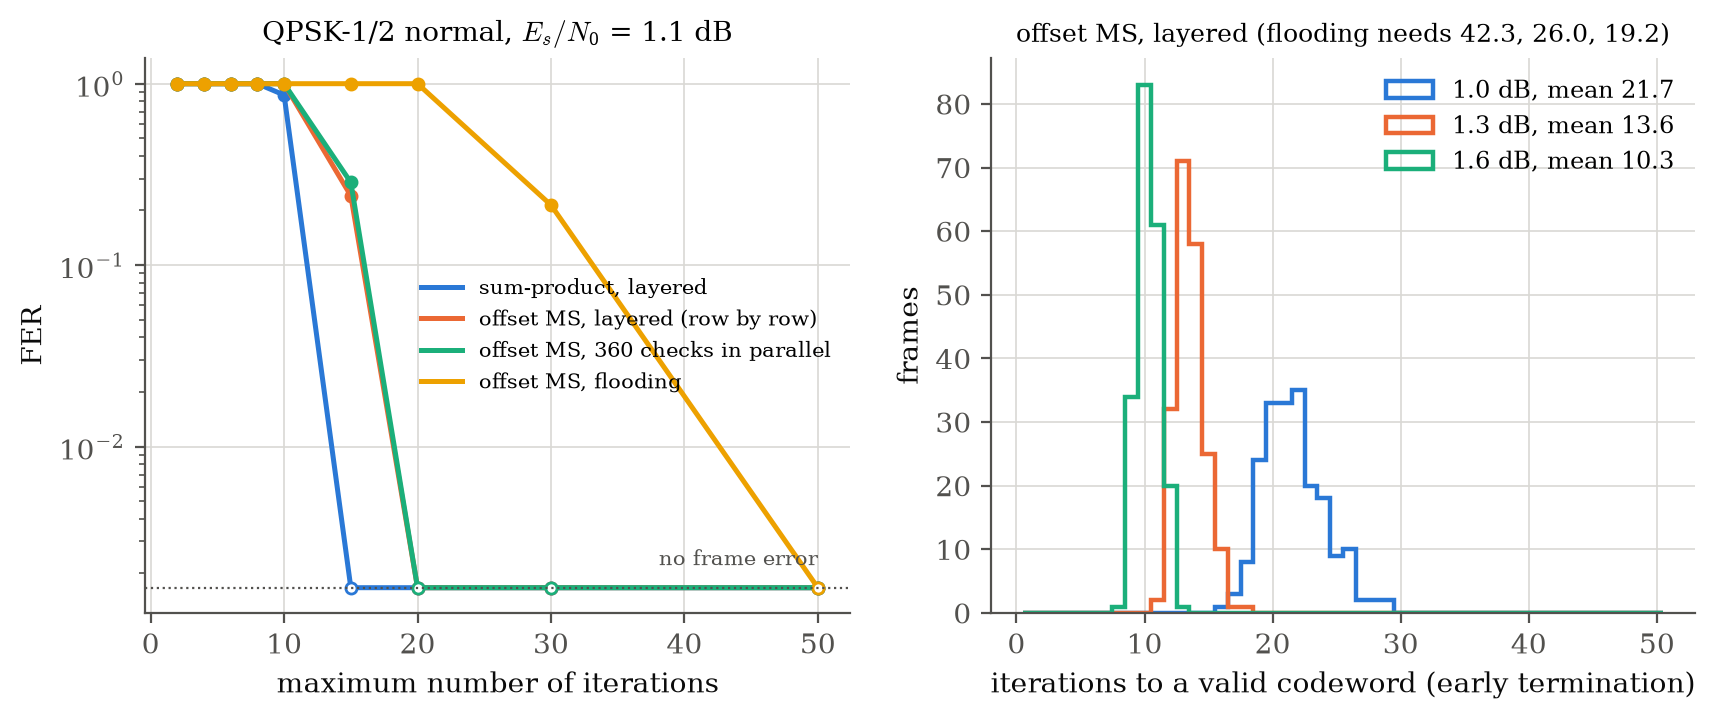
\includegraphics[width=\linewidth]{figures/ldpc-convergence.png}
\caption{Left: FER versus the maximum number of iterations for QPSK 1/2 normal frames at 1.1 dB. Right: number of iterations that the layered offset min-sum decoder needs to reach a codeword when it stops on a zero syndrome.} \label{fig:ldpc-convergence}
\end{figure}

Figure~\ref{fig:ldpc-convergence} measures the difference on QPSK 1/2 normal frames, 0.2 dB above the point where sum-product decoding reaches FER \(= 10^{-2}\) (up to 300 frames per point). With offset min-sum, the layered decoder decodes every frame within 20 iterations, while the flooding decoder still loses 21\% of the frames with 30 iterations and needs 50. When the decoder stops on a zero syndrome, the layered schedule needs on average 21.7, 13.6 and 10.3 iterations at 1.0, 1.3 and 1.6 dB, and the flooding schedule needs 42.3, 26.0 and 19.2: almost exactly twice as many. Sum-product decoding converges a few iterations faster than offset min-sum (13.6 iterations on average at 1.1 dB, against 17.6), but each iteration costs much more.

Two variants of the layered decoder are compared in the figure: one processes the checks one by one in natural order (\texttt{oms}), the other processes the 360 checks of a layer simultaneously, as the hardware of Section~\ref{sec:ldpc-arch} does, with the additive update for weight-2 circulants (\texttt{hw-oms}). Their curves are on top of each other: 17.6 against 17.8 iterations on average, and FER 0.24 against 0.29 when they are stopped after 15 iterations. Processing a whole layer in parallel therefore costs nothing measurable.

The distribution of the iterations is narrow: at 1.3 dB no frame needs more than 18 iterations with the layered decoder, against an average of 13.6. A decoder dimensioned for the average rather than the maximum number of iterations, with an input buffer that absorbs the occasional slow frame, is about twice as fast as one dimensioned for the worst case (Section~\ref{sec:ldpc-perf}).

\section{Structure of the DVB-S2 Code} \label{sec:ldpc-qc}

The DVB-S2 codes have a 360-periodic structure, and hardware decoders exploit it \cite{b:KienleDVBS2, b:UrardDVBS2}. Recall the encoding rule of Section~\ref{sec:LDPCstruct}: information bit \(i = 360 g + l\) (group \(g\), position \(0 \le l < 360\)) is added to the parity accumulators
\begin{equation} \label{eq:ldpc-address}
(x + l\,q) \bmod (N - K) \virgola \qquad x \in \text{row } g \text{ of the address table} \virgola \qquad q = \frac{N - K}{360}
\end{equation}
Write every check index as \(r = a + b\,q\) with \(0 \le a < q\) and \(0 \le b < 360\), and renumber it
\begin{equation} \label{eq:ldpc-perm}
r' = 360\,a + b
\end{equation}
An address \(x = a + b\,q\) sends information bit \(l\) of group \(g\) to check \((x + l q) \bmod (N - K) = a + \big((b + l) \bmod 360\big) q\), that is, to row \((l + b) \bmod 360\) of block row \(a\) in the new numbering. Within the \(360 \times 360\) block at block row \(a\) and block column \(g\), column \(l\) has its 1 in row \((l + b) \bmod 360\). This is the identity matrix cyclically shifted by \(b\), a \emph{circulant} \(\vet P^b\). The parity bits are renumbered in the same way. Parity bit \(j = a + b q\) is checked by rows \(j\) and \(j + 1\) (the staircase of Section~\ref{sec:LDPCstruct}), and these become an identity in block \((a, a)\), an identity in block \((a+1, a)\) and, for \(a = q - 1\), the circulant \(\vet P^1\) in block \((0, q-1)\) with its wrap-around entry missing, because parity bit \(N - K - 1\) has no successor. After the permutation the whole parity-check matrix is a \(q \times (N/360)\) array of circulants:
\begin{equation} \label{eq:ldpc-qc}
\vet H' = \begin{pmatrix}
\vet P^{b_{0,0}} & \cdots & & \vet I & & & \vet P^1_{-} \\
\vdots & \ddots & & \vet I & \vet I & & \\
& & & & \ddots & \ddots & \\
\cdots & & \vet P^{b_{q-1,g}} & & & \vet I & \vet I
\end{pmatrix}
\end{equation}
where a block is either zero or a shifted identity, and \(\vet P^1_{-}\) denotes the special parity block. Figure~\ref{fig:ldpc-qc} shows the transformation on the short rate 1/2 code. On the left is \(\vet H\) as defined by the standard. In the middle are the same rows and columns renumbered, and the matrix falls apart into diagonal segments. On the right are the circulants of one block row.

\begin{figure} \centering
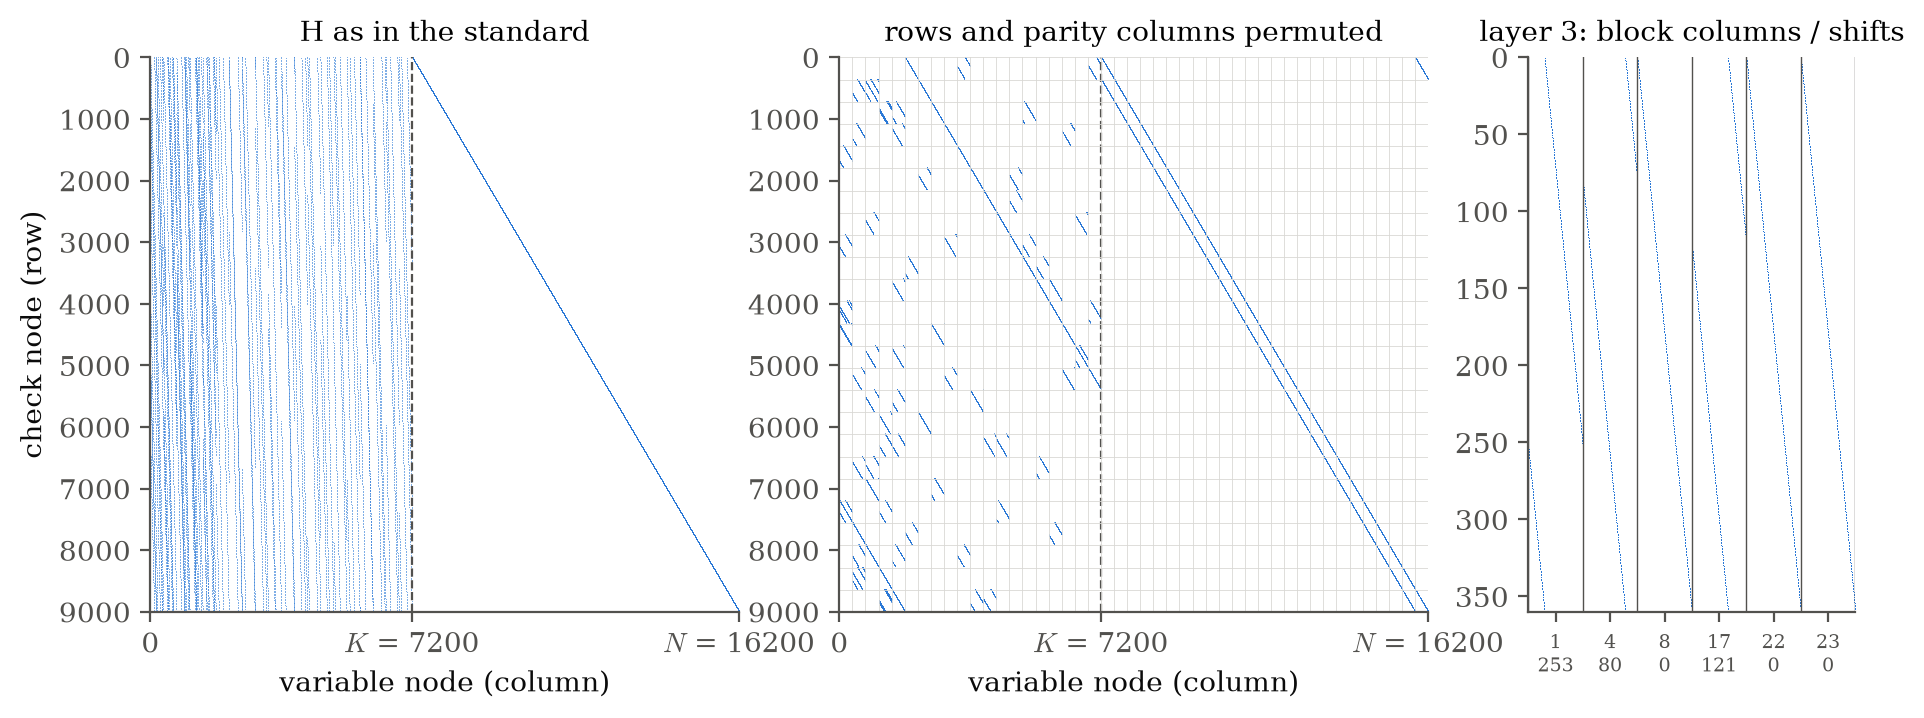
\includegraphics[width=\linewidth]{figures/ldpc-qc-structure.png}
\caption{The parity-check matrix of the short rate 1/2 DVB-S2 code (9000 checks, 16\,200 bits) as defined by the standard (left) and after the renumbering (\ref{eq:ldpc-perm}) of the checks and parity bits (middle; the grid marks the \(360 \times 360\) blocks). Right: block row 3, made of seven circulants; the tick labels give the block column and the shift.} \label{fig:ldpc-qc}
\end{figure}

A block row is a \emph{layer} of 360 checks. Each nonzero block is a permutation matrix, so each of its bits is checked once by the layer, and the 360 checks of a layer can be processed in parallel by 360 check-node processors. For example, the first row of the normal rate 1/2 table starts with the addresses 54 and 9318, and \(q = 90\). Address 54 gives layer \(54 \bmod 90 = 54\) and shift \(\lfloor 54 / 90 \rfloor = 0\). Address 9318 gives layer 48 and shift 103. Each address of the table becomes exactly one entry of a "block column, shift" list per layer. This list is the only code-dependent information the decoder needs, and its size is a few kilobits (Table~\ref{tb:ldpc-memory}).

There is one exception to "one bit, one check per layer". When two addresses of the same table row are congruent modulo \(q\), two circulants of the same information block column fall in the same layer, and every bit of that block column meets two checks of the layer. These \emph{weight-2 circulants} appear in every DVB-S2 code, from 3 in the normal rate 1/4 code to 39 in the normal rate 5/6 code (Table~\ref{tb:ldpc-structure}). The decoder handles them with the additive update (\ref{eq:ldpc-layer3}): the block column is read once and fed to two shifters, and the two message changes are summed before the write-back. Section~\ref{sec:ldpc-layered} showed that this costs nothing measurable.

\begin{table} \centering
\begin{tabular}{|l|c|c|c|c|c|c|}
\hline
frame & rate & layers \(q\) & \(K/360\) & check degree & circulants & weight-2 \\
\hline
normal & 1/4 & 135 & 45 & 4 & 540 & 3 \\
normal & 1/3 & 120 & 60 & 5 & 600 & 13 \\
normal & 2/5 & 108 & 72 & 6 & 648 & 8 \\
normal & 1/2 & 90 & 90 & 7 & 630 & 8 \\
normal & 3/5 & 72 & 108 & 11 & 792 & 35 \\
normal & 2/3 & 60 & 120 & 10 & 600 & 12 \\
normal & 3/4 & 45 & 135 & 14 & 630 & 23 \\
normal & 4/5 & 36 & 144 & 18 & 648 & 34 \\
normal & 5/6 & 30 & 150 & 22 & 660 & 39 \\
normal & 8/9 & 20 & 160 & 27 & 540 & 30 \\
normal & 9/10 & 18 & 162 & 30 & 540 & 36 \\
short & 1/4 & 36 & 9 & 4 & 135 & 4 \\
short & 1/3 & 30 & 15 & 5 & 150 & 4 \\
short & 2/5 & 27 & 18 & 6 & 162 & 8 \\
short & 1/2 & 25 & 20 & 4--7 & 135 & 8 \\
short & 3/5 & 18 & 27 & 11 & 198 & 27 \\
short & 2/3 & 15 & 30 & 10 & 150 & 14 \\
short & 3/4 & 12 & 33 & 9--13 & 132 & 9 \\
short & 4/5 & 10 & 35 & 11--13 & 125 & 9 \\
short & 5/6 & 8 & 37 & 15--19 & 137 & 21 \\
short & 8/9 & 5 & 40 & 27 & 135 & 20 \\
\hline
\end{tabular}
\caption{Quasi-cyclic structure of the DVB-S2 LDPC codes after the permutation (\ref{eq:ldpc-perm}). \(K/360\) is the number of information block columns. "Circulants" counts the nonzero \(360 \times 360\) blocks, including the parity part. Each edge of the Tanner graph belongs to exactly one of them, so the number of edges is \(360 \times\) circulants \(- 1\), the missing entry of \(\vet P^1_-\). Check degrees are listed as a range where they vary by more than the single missing edge of the first check.} \label{tb:ldpc-structure}
\end{table}

The number 360 is the same one that sets the parallelism of the LDPC encoder in Chapter~\ref{ch:BCHencImpl}: the encoder adds 360 information bits per clock cycle to the parity accumulators, and the BCH encoder of this thesis was given \(p = 8\), a divisor of 360, so that its output fills the LDPC input memory in words of 360 bits. The decoder uses the same structure: one memory word holds the 360 bits of one block column.

\section{Decoder Architecture} \label{sec:ldpc-arch}

\begin{figure} \centering
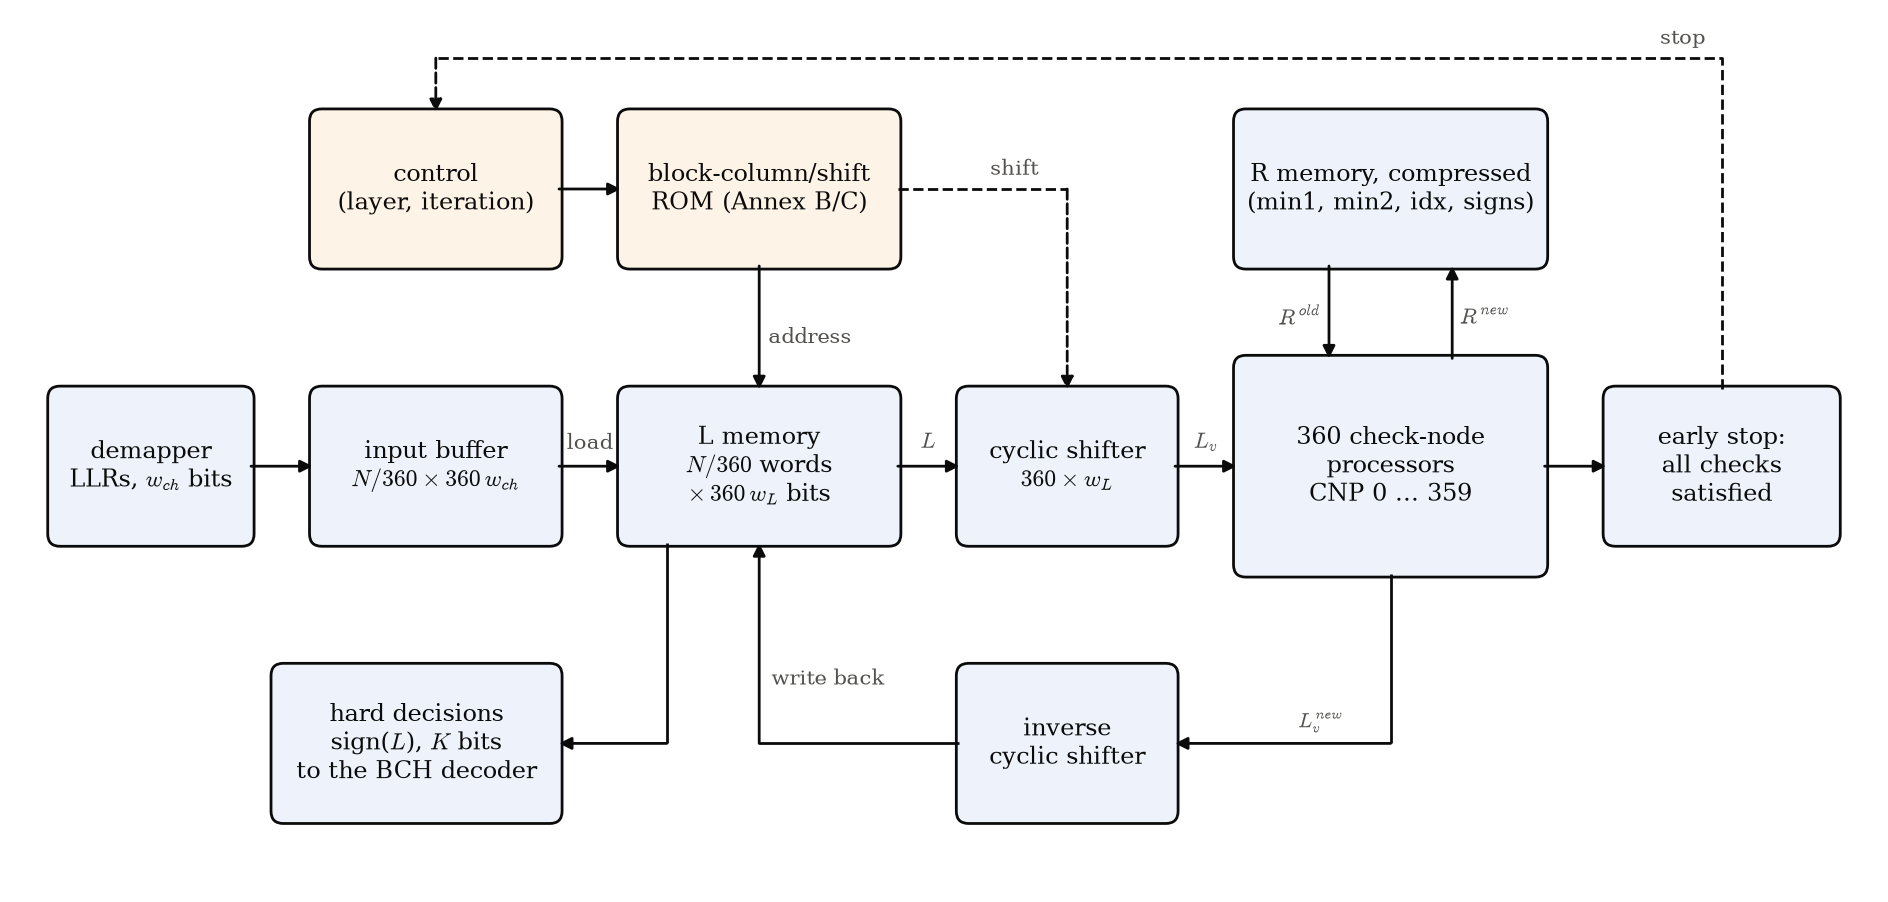
\includegraphics[width=\linewidth]{figures/ldpc-decoder-architecture.png}
\caption{Top-level architecture of the layered LDPC decoder with 360 check-node processors. Solid lines: data; dashed lines: control.} \label{fig:ldpc-arch}
\end{figure}

Figure~\ref{fig:ldpc-arch} shows the proposed architecture. It is a partially parallel layered decoder built from the following parts.

\begin{description}
\item[Input buffer] It holds the channel LLRs of the next frame (\(N\) values of \(w_{ch}\) bits) while the current frame is decoded, so decoding and reception overlap.
\item[L memory] It holds the posteriors \(L_v\) as \(N/360\) words of \(360 \times w_L\) bits: word \(g\) contains block column \(g\). It is loaded from the input buffer at the start of a frame, in \(N/360\) cycles.
\item[Block-column/shift ROM] For each layer it holds the list of nonzero blocks: block column (address of the L-memory word) and shift. It is built from the address table of the standard (Annexes B and C) for every code rate. Changing the rate means changing the ROM page, so the datapath is the same for all 21 codes.
\item[Cyclic shifters] The CNP for row \(b\) of a layer needs bit \((b - s) \bmod 360\) of a block with shift \(s\), so the word read from L memory is rotated by \(s\) before it reaches the processors, and rotated back by \(-s\) before it is written. A barrel shifter of \(360 \times w_L\) bits does this in \(\lceil \log_2 360 \rceil = 9\) stages of multiplexers.
\item[Check-node processors] 360 identical processors (CNPs), one per row of the layer, each processing one edge per clock cycle (Figure~\ref{fig:ldpc-cnp}).
\item[R memory] It holds the compressed state (\ref{eq:ldpc-compressed}) of every check: one word of \(360\) states per layer.
\item[Early stop] It accumulates the parity of every check from the signs of the updated \(L_v\) and stops the decoder when an iteration ends with all checks satisfied. A simpler check, as here, verifies the full syndrome after the iteration.
\item[Output buffer] It holds the \(K\) hard decisions \(\mathrm{sign}(L_v)\) of the information part, which go to the BCH decoder.
\end{description}

\paragraph{Check-node processor.} Figure~\ref{fig:ldpc-cnp} shows the datapath of one CNP. Processing a layer takes two phases of \(d_c\) cycles each, one per block column. In the \emph{read} phase the CNP receives \(L_v\) and decompresses \(R_{c \to v}\ap{old}\) from the state it stored one iteration earlier. It forms \(Q = \mathrm{sat}(L_v - R\ap{old})\) as in (\ref{eq:ldpc-layer1}), pushes \(Q\) into a FIFO, and updates a running two-minimum search (\(m_1\), \(m_2\), index of \(m_1\)) and the parity of the signs. At the end of the phase the offset (\ref{eq:ldpc-corrections}) is applied to \(m_1\) and \(m_2\), and the new state goes to the R memory. In the \emph{write} phase the CNP pops each \(Q\), selects \(m_1\) or \(m_2\) and the sign, and writes \(L_v = \mathrm{sat}(Q + R\ap{new})\) as in (\ref{eq:ldpc-layer3}). The two-minimum finder is two comparators and two registers. Apart from the shifters, the whole decoder needs no multiplier and no lookup table.

\begin{figure} \centering
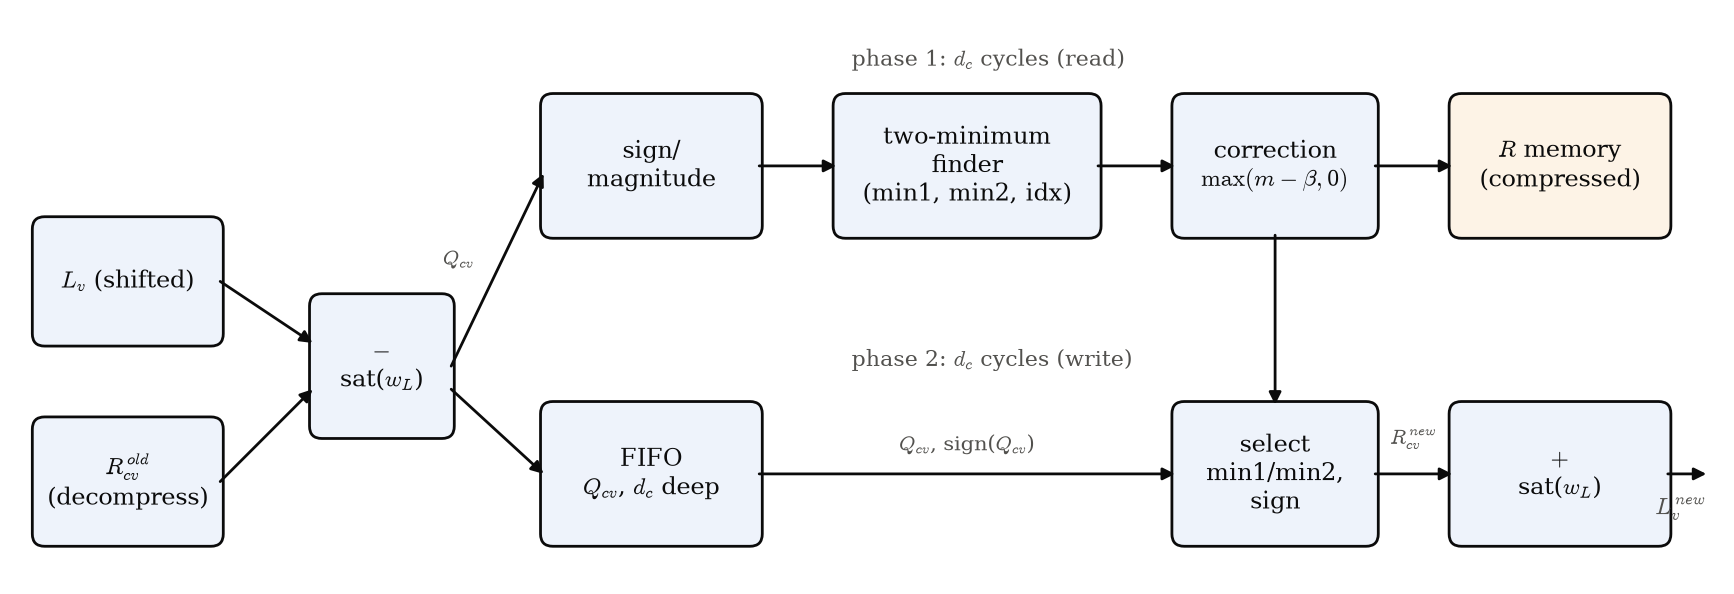
\includegraphics[width=\linewidth]{figures/ldpc-cnp.png}
\caption{Datapath of one check-node processor for offset min-sum. The read phase computes the new compressed state of the check; the write phase updates the posteriors.} \label{fig:ldpc-cnp}
\end{figure}

\paragraph{Pipelining and hazards.} If the two phases of a layer and the pipeline between them (\(D\) cycles: memory read latency, shifter, subtraction, minimum search, correction) run one after the other, a layer takes \(2 d_c + D\) cycles and the datapath is idle half of the time. The obvious improvement is to start reading layer \(\ell + 1\) while layer \(\ell\) is still being written. This creates a \emph{read-after-write hazard}: if a block column of layer \(\ell + 1\) is also in layer \(\ell\), it may be read only after layer \(\ell\) has written it back, otherwise layer \(\ell + 1\) works on a stale \(L_v\). In natural order this happens all the time, because consecutive layers \(a\) and \(a + 1\) always share a parity block column (the staircase), and the decoder must stall. Figure~\ref{fig:ldpc-pipeline} shows the first layers of the short rate 1/2 code with \(D = 4\).

Layered decoding is correct in any layer order, and the block columns inside a layer can also be processed in any order. Two reorderings remove most of the stalls:
\begin{enumerate}
\item visit the layers in an order where consecutive layers share as few block columns as possible (a greedy search: from the current layer, go to the unvisited layer with the fewest shared block columns);
\item within each layer, read last the block columns that the previous layer writes, and read first (and therefore write first) those that the next layer needs.
\end{enumerate}
Table~\ref{tb:ldpc-cycles} counts the cycles per iteration for the normal codes with \(D = 6\) in the three cases. The model is \texttt{architecture()} in \texttt{ldpc\_hw.py}; it schedules the reads cycle by cycle and inserts a stall wherever a block column would be read before it is written. With reordering, 6 of the 11 codes reach the lower bound of one cycle per distinct block column and layer, and the others come within 0.3--6.1\%.

\begin{figure} \centering
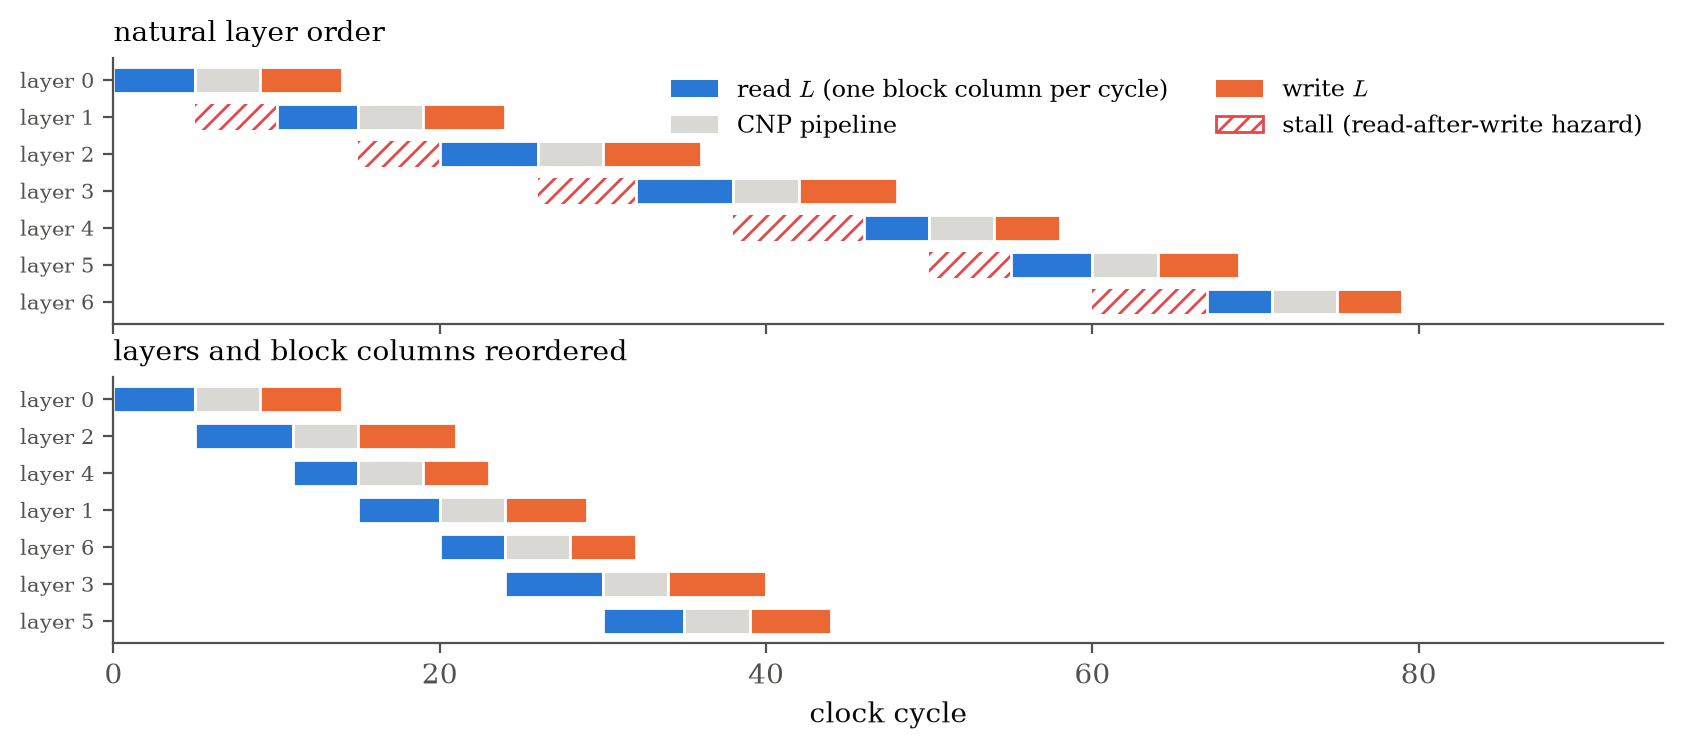
\includegraphics[width=\linewidth]{figures/ldpc-pipeline.png}
\caption{Pipelined processing of the first seven layers of the short rate 1/2 code (pipeline depth \(D = 4\)). In natural order (top) consecutive layers share block columns and the pipeline stalls. With the layer and block-column order chosen to separate them (bottom) there are no stalls.} \label{fig:ldpc-pipeline}
\end{figure}

\begin{table} \centering
\begin{tabular}{|c|c|c|c|c|c|c|c|}
\hline
rate & bound & serial & overlapped & reordered & \multicolumn{2}{c|}{Mb/s, 30 it.} & latency \\
 & & & (stalls) & (stalls) & serial & reordered & [\(\mu\)s] \\
\hline
1/4 & 537 & 1884 & 1615 (1078) & 545 (8) & 57 & 196 & 82.7 \\
1/3 & 587 & 1894 & 1546 (959) & 591 (4) & 76 & 241 & 89.5 \\
2/5 & 640 & 1928 & 1502 (862) & 642 (2) & 89 & 267 & 97.2 \\
1/2 & 622 & 1784 & 1341 (719) & 622 (0) & 121 & 344 & 94.2 \\
3/5 & 757 & 1946 & 1339 (582) & 757 (0) & 133 & 340 & 114.5 \\
2/3 & 588 & 1536 & 1069 (481) & 588 (0) & 187 & 485 & 89.1 \\
3/4 & 607 & 1484 & 970 (363) & 607 (0) & 217 & 529 & 92.0 \\
4/5 & 614 & 1444 & 911 (297) & 614 (0) & 238 & 557 & 93.0 \\
5/6 & 621 & 1422 & 869 (248) & 659 (38) & 252 & 541 & 99.8 \\
8/9 & 510 & 1140 & 673 (163) & 510 (0) & 335 & 744 & 77.4 \\
9/10 & 504 & 1116 & 656 (152) & 507 (3) & 347 & 758 & 77.0 \\
\hline
\end{tabular}
\caption{Clock cycles per iteration of the 360-CNP decoder for normal frames with pipeline depth \(D = 6\). "Bound" is the number of distinct block columns summed over the layers (one read per cycle); "serial" processes one layer at a time; "overlapped" starts each layer while the previous one writes, in natural order; "reordered" also reorders layers and block columns. Information throughput and latency at 200 MHz and 30 iterations, including the \(N/360\) cycles that load a frame.} \label{tb:ldpc-cycles}
\end{table}

\paragraph{Partial parallelism.} The number of processors \(P\) can be any divisor of 360. Each block column is then processed in \(360/P\) slices of \(P\) rows, and the cycle counts scale by \(360/P\). The memories keep their size but become \(360/P\) times narrower and deeper. One complication is that the shift of a circulant moves bits between slices, so the shifter must combine two adjacent memory words. Figure~\ref{fig:ldpc-parallelism} shows the throughput versus \(P\). The choice of \(P\) is a trade-off between area and the symbol rate the modem must support (Section~\ref{sec:ldpc-perf}).

\begin{figure} \centering
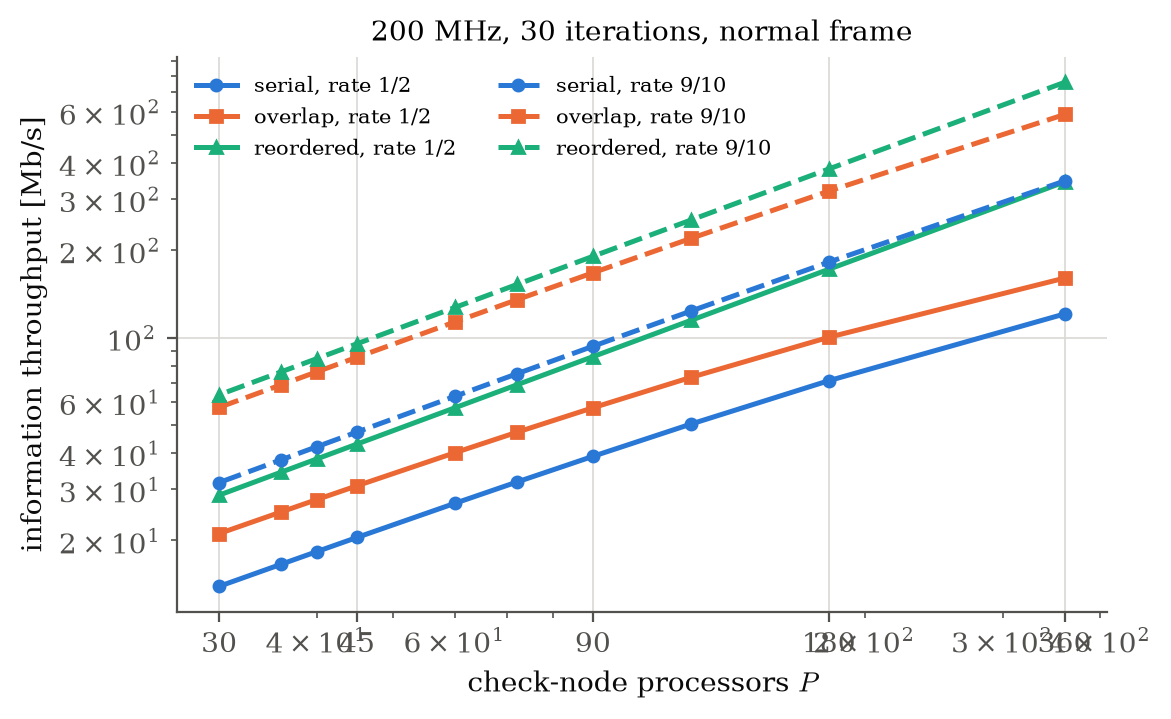
\includegraphics[width=0.75\linewidth]{figures/ldpc-parallelism.png}
\caption{Information throughput versus the number of check-node processors for the normal rate 1/2 and 9/10 codes (200 MHz, 30 iterations, pipeline depth 6) with the three schedules of Table~\ref{tb:ldpc-cycles}.} \label{fig:ldpc-parallelism}
\end{figure}

\section{Finite Precision} \label{sec:ldpc-fixed}

The hardware works on integers. The bit-true model (\texttt{FixedPoint} and \texttt{layer\_decode} in \texttt{ldpc\_hw.py}) reproduces the datapath of Figure~\ref{fig:ldpc-cnp} exactly. It has a vectorized numpy version and a compiled numba version, and the tests check that the two agree bit for bit. Its parameters are:
\begin{description}
\item[\(w_{ch}\)] the width of the channel LLRs. The demapper output is multiplied by a scale \(s\) (LSBs per LLR unit), rounded to the nearest integer and saturated to \(\pm(2^{w_{ch}-1} - 1)\).
\item[\(w_L\)] the width of the posteriors \(L_v\) and of \(Q\). Both are saturated after every addition or subtraction.
\item[\(w_R\)] the width of the check messages: a sign and \(w_R - 1\) magnitude bits.
\item[\(\beta\)] the offset in LSBs. With \(s = 2\), \(\beta = 1\) LSB is the \(\beta = 0.5\) of Section~\ref{sec:ldpc-minsum}. A normalization \(\alpha = A/2^k\) is computed as \(\lfloor A\,m / 2^k \rfloor\).
\end{description}
The notation \((w_{ch}, w_L, w_R)\) is used below. The posterior needs more bits than the channel LLR because it accumulates up to \(d_v\) check messages, and \(L_v\) must saturate gracefully when a bit is already certain.

\begin{figure} \centering
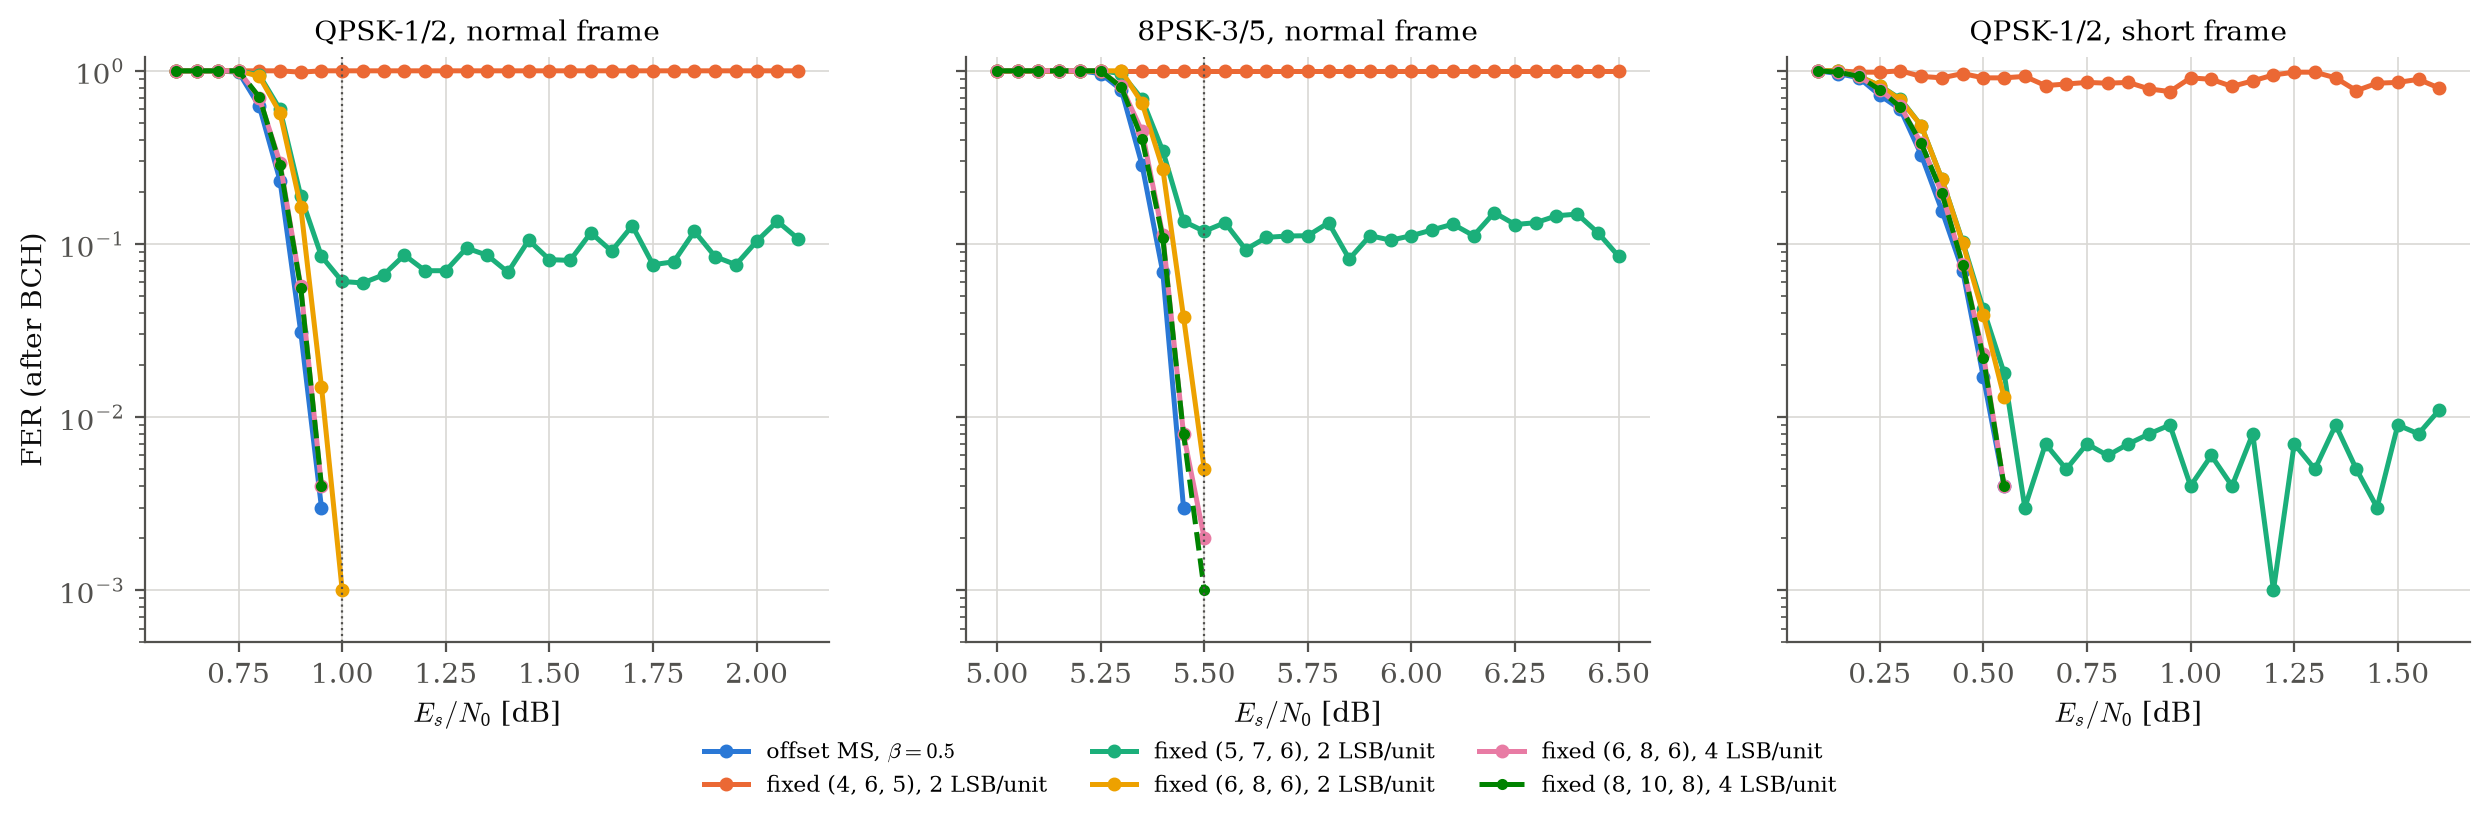
\includegraphics[width=\linewidth]{figures/ldpc-quantization.png}
\caption{Frame error rate after BCH of the bit-true fixed-point decoder (offset min-sum, layered, 50 iterations) for several word lengths \((w_{ch}, w_L, w_R)\) and scales, against the floating-point offset min-sum decoder.} \label{fig:ldpc-quantization}
\end{figure}

Figure~\ref{fig:ldpc-quantization} compares several formats on three MODCODs, and Table~\ref{tb:ldpc-headroom} isolates the decisive parameter. Four observations shape the design.

\paragraph{The posterior needs two bits of headroom.} With \(w_L = w_R + 1\) the decoder either has an error floor that does not improve with the signal-to-noise ratio (\(w_R = 6\): FER \(\approx 0.1\) on normal frames, \(\approx 5 \cdot 10^{-3}\) on the short frame) or fails altogether (\(w_R = 5\)), and with \(w_L \le w_R\) it never decodes. The failed frames have tens of thousands of wrong bits: the decoder diverges rather than converging to a wrong codeword. With \(w_L \ge w_R + 2\) every frame is decoded, whatever the channel resolution. The mechanism is the bookkeeping of (\ref{eq:ldpc-layer1})--(\ref{eq:ldpc-layer3}). When \(L_v\) saturates, it no longer equals \(\lambda_v + \sum_c R_{c \to v}\), and the subtraction \(Q = L_v - R\ap{old}\) removes a message that was never fully added. If one check then changes its mind, \(L_v = Q + R\ap{new}\) can fall close to zero, even though all the other checks of the bit agree. With two extra bits, the posterior can hold four full-scale messages before it saturates.

\paragraph{Six bits of channel LLR are enough.} \((6, 8, 6)\) at \(s = 4\) LSBs per LLR unit and \(\beta = 2\) LSBs (the \(\beta = 0.5\) of Section~\ref{sec:ldpc-minsum}) gives exactly the thresholds of the floating-point decoder on all three codes, and so does the wider \((8, 10, 8)\). At \(s = 2\) and \(\beta = 1\) LSB the loss is 0.05 dB. Although the channel LLRs then saturate at \(\pm 7.75\), the finer resolution of small messages matters more than the range of large ones. Large LLRs are reliable anyway.

\paragraph{A normalization in fixed point is also an offset.} \(\lfloor 7m/8 \rfloor\) maps \(m = 1\) to 0 and \(m = 2\) to 1, so at a coarse scale the truncation subtracts up to one LSB from every message. On the normal frames, \((6, 8, 6)\) with \(\alpha = 7/8\) at \(s = 2\) is 0.10--0.20 dB better than the same normalization on a fine grid (\(s = 32\)), which behaves like the floating-point normalized decoder. On the short frame the effect is reversed (0.25 dB worse). The truncation is an uncontrolled offset, and it is better to make the offset explicit.

\paragraph{Memory.} With \((6, 8, 6)\) the L memory holds \(8N\) bits and the compressed R memory \(10 + \lceil\log_2 d_c\rceil + d_c\) bits per check (Table~\ref{tb:ldpc-memory}). One more bit in \(w_L\) costs 65 kbit for normal frames; one fewer would put the decoder on the error floor of Table~\ref{tb:ldpc-headroom}.

\begin{table} \centering
\begin{tabular}{|c|c|c|c|}
\hline
\((w_{ch}, w_L, w_R)\) & \(w_L - w_R\) & QPSK 1/2, 1.5 dB & 8PSK 3/5, 5.9 dB \\
\hline
(4, 5, 5) & 0 & 1 & 1 \\
(4, 6, 5) & 1 & 1 & 1 \\
(4, 7, 5) & 2 & 0 & 0 \\
(4, 8, 5) & 3 & 0 & 0 \\
(5, 6, 6) & 0 & 1 & 1 \\
(5, 7, 6) & 1 & 0.081 & 0.112 \\
(5, 8, 6) & 2 & 0 & 0 \\
(5, 9, 6) & 3 & 0 & 0 \\
\hline
\end{tabular}
\caption{Frame error rate of the fixed-point decoder (\(s = 2\), offset 1 LSB, normal frames) 0.6 dB above the sum-product threshold, well beyond the waterfall of the floating-point decoders (Figure~\ref{fig:ldpc-algorithms}). "0" means no error in 1000 frames. The results with \(w_{ch} = w_R\) are practically the same.} \label{tb:ldpc-headroom}
\end{table}

\section{Throughput, Latency and Memory} \label{sec:ldpc-perf}

With \(P\) processors, \(C\) cycles per iteration at \(P = 360\) (Table~\ref{tb:ldpc-cycles}), \(I\) iterations and clock frequency \(f\), one frame takes
\begin{equation} \label{eq:ldpc-throughput}
T\ped{frame} = \frac{1}{f}\left( I\,C\,\frac{360}{P} + \frac{N}{P} \right) \virgola \qquad \text{throughput} = \frac{K}{T\ped{frame}}
\end{equation}
and the latency is \(T\ped{frame}\) plus the time to receive the frame. The decoder must keep up with the symbol rate \(R_s\) of the modem: it must deliver \(R_s \eta\) information bits per second, where \(\eta\) is the spectral efficiency of the MODCOD. At \(R_s = 30\) Mbaud, a typical 36 MHz transponder, this is 30 Mb/s for QPSK 1/2 and 134 Mb/s for 32APSK 9/10. Over the 28 MODCODs with normal frames, the 360-CNP decoder at 200 MHz and 30 iterations (Table~\ref{tb:ldpc-cycles}) exceeds this requirement by a factor between 4.4 (32APSK 5/6) and 14 (QPSK 9/10), so a smaller decoder suffices. With \(P = 90\) (Figure~\ref{fig:ldpc-parallelism}) the reordered decoder still delivers 86 Mb/s at rate 1/2 and 191 Mb/s at rate 9/10, and it meets 30 Mbaud at every MODCOD with a quarter of the processors. The tightest case is 32APSK 5/6, which needs 124 Mb/s and gets 141 Mb/s. Because the average number of iterations is much smaller than the maximum (Figure~\ref{fig:ldpc-convergence}), an input buffer of two frames lets the decoder spend more iterations on the occasional difficult frame without lowering the average throughput.

The binding MODCODs are the 32APSK ones with rates 3/4 to 5/6, which combine a high spectral efficiency with codes of moderate rate. Low-rate codes are slow in bits per second, but the MODCODs that use them carry little information. They are also where the schedule matters most: they have the most layers and the smallest check degrees, so in the serial schedule the pipeline latency of every layer dominates. At rate 1/4 the reordered schedule is 3.4 times faster than the serial one.

\begin{table} \centering
\begin{tabular}{|c|c|c|c|c|c|c|c|}
\hline
rate & L & R compressed & R full & input buffer & output & ROM & total \\
\hline
1/4 & 518 & 778 & 1166 & 389 & 16 & 9.2 & 1710 \\
1/3 & 518 & 778 & 1296 & 389 & 22 & 10.2 & 1717 \\
2/5 & 518 & 739 & 1400 & 389 & 26 & 11.0 & 1683 \\
1/2 & 518 & 648 & 1361 & 389 & 32 & 10.7 & 1598 \\
3/5 & 518 & 648 & 1711 & 389 & 39 & 13.5 & 1608 \\
2/3 & 518 & 518 & 1296 & 389 & 43 & 10.2 & 1479 \\
3/4 & 518 & 454 & 1361 & 389 & 49 & 10.7 & 1420 \\
4/5 & 518 & 428 & 1400 & 389 & 52 & 11.0 & 1398 \\
5/6 & 518 & 400 & 1426 & 389 & 54 & 11.2 & 1372 \\
8/9 & 518 & 302 & 1166 & 389 & 58 & 9.2 & 1276 \\
9/10 & 518 & 292 & 1166 & 389 & 58 & 9.2 & 1266 \\
\hline
\end{tabular}
\caption{Memory of the decoder in kbit for normal frames with \((w_{ch}, w_L, w_R) = (6, 8, 6)\). "R full" would store every message instead of the compressed state (\ref{eq:ldpc-compressed}); the total uses the compressed state. "Output" holds the \(K\) decoded bits for the BCH decoder; "ROM" holds the block column and shift of every circulant (\(\lceil\log_2(N/360)\rceil + 9\) bits each).} \label{tb:ldpc-memory}
\end{table}

Table~\ref{tb:ldpc-memory} lists the memories. A decoder that supports every rate needs the largest of each column: about 0.52 Mbit of L memory, 0.78 Mbit of R memory (rate 1/4 and 1/3, which have the most checks), 0.39 Mbit of input buffer and 58 kbit of output buffer, about 1.75 Mbit in all, plus 11 ROM pages of at most 13.5 kbit each. The R memory would be 1.71 Mbit without the compression of Section~\ref{sec:ldpc-minsum}. This size fits in the embedded memory of a large FPGA, such as the Stratix II EP2S180 used for the transmitter in Chapter~\ref{ch:TestTXSec}, which has 9.4 Mbit, and is small for an ASIC.

For comparison, the BCH encoder of Chapter~\ref{ch:BCHencImpl} processes \(p = 8\) bits per cycle and needs \(K\ped{bch}/8\) cycles per frame, for example 4026 cycles for rate 1/2. The LDPC decoder at 30 iterations needs \(30 \times 622 + 180 \approx 18\,800\) cycles for the same frame with 360 processors, about 4.7 times more, even with 45 times the parallelism. Iterative decoding, not encoding, dominates the complexity of the DVB-S2 FEC. This is the reason the standard fixed the 360-periodic structure that makes the decoder parallel.

\section{Summary of the Design}

\begin{table} \centering
\begin{tabular}{|p{4cm}|p{9cm}|}
\hline
Choice & Reason \\
\hline
Offset min-sum, \(\beta = 0.5\) & Multiplier-free; 0.10--0.20 dB from sum-product (Table~\ref{tb:ldpc-thresholds}); the same \(\beta\) is best for all normal frames, while the best \(\alpha\) varies and a wrong one fails (Figure~\ref{fig:ldpc-correction}). \\
Layered schedule & About half the iterations of flooding (Figure~\ref{fig:ldpc-convergence}); no variable-to-check message memory. \\
360 CNPs, one layer of circulants per step & The renumbering (\ref{eq:ldpc-perm}) turns every DVB-S2 code into \(360 \times 360\) circulants; weight-2 circulants are resolved by adding the message changes. \\
Reordered layers and block columns & Removes the read-after-write stalls of the overlapped pipeline: up to 3.5 times fewer cycles than serial processing (Table~\ref{tb:ldpc-cycles}). \\
Compressed check state & \(m_1\), \(m_2\), index and signs: 1.5--4 times less R memory. \\
\((w_{ch}, w_L, w_R) = (6, 8, 6)\), \(s = 4\) & Same thresholds as floating point with \(\beta = 2\) LSB; the posterior needs two bits more than the messages, otherwise the decoder diverges (Table~\ref{tb:ldpc-headroom}). \\
\(P\) a divisor of 360 & Trades area for throughput; \(P = 90\) is enough for 30 Mbaud at every MODCOD with 30 iterations. \\
\hline
\end{tabular}
\caption{Design choices for the DVB-S2 LDPC decoder and the results that support them.} \label{tb:ldpc-summary}
\end{table}

Table~\ref{tb:ldpc-summary} summarizes the design. The decoder is the receiver-side counterpart of the encoder studied in this thesis: the same 360-bit groups that let the transmitter encode 360 bits per cycle let the receiver run 360 check-node processors in parallel, and the same address tables that drive the encoder fill the ROM of the decoder.
